%----------------------------------------------------------------------------------------
%	PAKET-/ UND ANDERE DOKUMENT-IMPORTS
%----------------------------------------------------------------------------------------
\documentclass{scrartcl}   % Formateinstellungen
\usepackage[ngerman]{babel} % deutsche Silbentrennung
\usepackage[utf8]{inputenc} % deutsche Umlaute
\usepackage{placeins}   % verbessert Anzeige eines Floats hinter dem Befehl \FloatBarrier
\usepackage{amsfonts}   % neue Schriftanpassungen (wird von amssymb (s.u.) geladen)
\usepackage{amssymb}    % erweitert Benutzung von amsfonts (s.o.)
\usepackage{amsmath}    % Vielzahl von neuen mathematischen Umgebungen und Befehlen (wird von mathtools (s.u.) geladen)
\usepackage{mathtools}  % Verbesserung von amsmath (s.o.)
\usepackage{booktabs}   % Tabellen ohne vertikale Striche
\usepackage{siunitx}    % Einheitensystem
\usepackage[margin={0.3cm,0.3cm},font=singlespacing,labelfont=bf,labelsep=endash]{caption} % Bildunterschriften
\usepackage{wrapfig}    % Bild von Text umfließen lassen
\usepackage{sidecap}    % ermöglicht Überschriften neben Bildern / Tabellen
\usepackage{setspace}   % zum Definieren des Zeilenabstandes
\usepackage{eurosym}    % ergänzt optimales Euro-Zeichen
\usepackage[perpage,marginal]{footmisc} % ermöglicht Fußnoten und das Verändern dieser
\usepackage{graphicx}   % ermöglicht besseres Einbinden von Grafiken
\usepackage{fancyhdr}   % zum Erstellen von Kopf- und Fußzeilen
\usepackage{listings}   % ermöglicht Quellcodelisting
\usepackage{color}  % Farb-Management von Vorder- und Hintergrundfarben
\usepackage{pdfpages}   % ermöglicht das Einbinden von ganzen oder nur Teilen von PDFs
\usepackage{lineno} % Zeilenzählung
\usepackage{framed} % ermöglicht das Einrahmen von Elementen
\usepackage{pifont} % fügt Symbol-Schriften hinzu
\usepackage[hidelinks]{hyperref}    % ermöglicht das Hinzufügen von Links und Verweisen innerhalb
                                    % des PDF Dokuments und weitere Einstellungen
\usepackage[left=2.5cm,right=2cm,top=2cm,bottom=2cm,includeheadfoot]{geometry}  % Größenanpassung der Seite
\usepackage{rotating} % ermöglicht Drehen von Bildern
%----------------------------------------------------------------------------------------


%----------------------------------------------------------------------------------------
%   KONFIGURATIONEN
%----------------------------------------------------------------------------------------
\begin{document}
\setlength{\parskip}{1ex}   % Abstand zwischen Absätzen 
\parindent 0pt  % legt Einrücke der ersten Zeile fest
\renewcommand{\thefigure}{\arabic{figure}.\alph{ab}}    % Umdefinieren von Bildnummern

\definecolor{darkblue}{rgb}{0,0,.6} % Festlegen der Farben
\definecolor{darkred}{rgb}{.6,0,0}  % Festlegen der Farben
\definecolor{darkgreen}{rgb}{0,.6,0}    % Festlegen der Farben
\definecolor{red}{rgb}{.98,0,0} % Festlegen der Farben
\definecolor{purple}{rgb}{0.44, 0.16, 0.39}  % Festlegen der Farben

\lstloadlanguages{Java} % lädt Programmiersprachen
\lstset{language=Java,basicstyle=\footnotesize\ttfamily,commentstyle=\itshape\color{darkgreen},keywordstyle=\bfseries\color{darkblue},stringstyle=\color{darkred},tabsize=3,showspaces=false,showtabs=false,columns=fixed,numbers=left,frame=single,numberstyle=\tiny,breaklines=true,showstringspaces=false,xleftmargin=1cm} % Erstellen eines Codeblocks
    
\pagestyle{fancy}   % Setzen des Seitenstyles "fancy" ermöglicht eigenes Erstellen einer Kopf- und Fußzeile
\fancyhf{}  % alle Kopf- und Fußzeilenfelder bereinigen
\fancyhead[L]{\leftmark}    % Kopfzeile links (mit "leftmark" erstellt man im Header das Chapter, mit "rightmark" die Section)
\fancyhead[C]{} % zentrierte Kopfzeile
\fancyhead[R]{\thepage} % Kopfzeile rechts
\fancypagestyle{plain}  % legt Seiten-Typen fest

\newcommand{\barrow}{\item[\ding{228}]} % hinzufügen des Pfeil-Aufzählsymbols unter dem Command \barrow
%----------------------------------------------------------------------------------------


%----------------------------------------------------------------------------------------
%   1. SEITE
%----------------------------------------------------------------------------------------
\titlehead{\Large

\begin{center}
\begin{framed}
\centering {Inoffizielle Lösungen und Erklärungen - \href{https://www.inf-schule.de/inf-schule}{inf-schule\textsuperscript{\textcopyright}} (\href{https://creativecommons.org/licenses/by-sa/4.0/legalcode.de}{\textit{Lizenz}})}

\centering {\Large\textbf{\href{https://inf-schule.de/programmierung/oopjava}{2.3 Objektorientierte Programmierung mit Java}}}
\end{framed}
\end{center}}

\title{\huge{\href{https://www.inf-schule.de/programmierung/oopjava/implementierung/spaceinvaders}{2.4\\Space Invaders}}\\
\vspace{0.5cm}
\begin{figure}[ht]
	\centering
	\href{https://creativecommons.org/licenses/by-sa/3.0/de/}{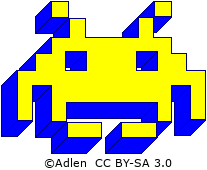
\includegraphics[height=4.5cm]{Space_Invaders.png}}
\end{figure}
\vspace{2cm}}

\author{\textbf{Benötigte IDEs:}\\
\href{https://www.greenfoot.org/}{Greenfoot}
\vspace{2cm}}

\date{\textbf{Verfasser:}\\
\href{https://nikothegreek.jimdofree.com/}{Cyb3rKo}\\
\vspace{0.5cm}
\textbf{Erstellungs-/ Änderungsdatum}\\
\today\enlargethispage{4cm}}
%----------------------------------------------------------------------------------------

%----------------------------------------------------------------------------------------
%   2. SEITE
%----------------------------------------------------------------------------------------
\doublespacing

\maketitle\thispagestyle{empty}

\numberwithin{equation}{section}
\cleardoublepage

\setcounter{page}{1}
\tableofcontents
%----------------------------------------------------------------------------------------


%----------------------------------------------------------------------------------------
%   3. UND NACHFOLGENDE SEITEN
%----------------------------------------------------------------------------------------
\newpage
\pagenumbering{arabic}  % Ändern der Seitenangabe

\cleardoublepage

\section{Spielbeschreibung}

Zu dieser Seite sind meines Erachtens nach keine Anleitungen und/oder Erläuterungen nötig.\\
Wenn doch Fragen aufkommen, schreib' einfach an \textbf{\href{mailto:niko@cyb3rko.de}{niko@cyb3rko.de}}.

\newpage

\section{Entwicklung des Spiels}

\subsection{Pflichtenheft}

Hier erstmal meine Skizze zu meiner Spiel-Idee:\\
\begin{figure}[ht]
\begin{turn}{-90}
	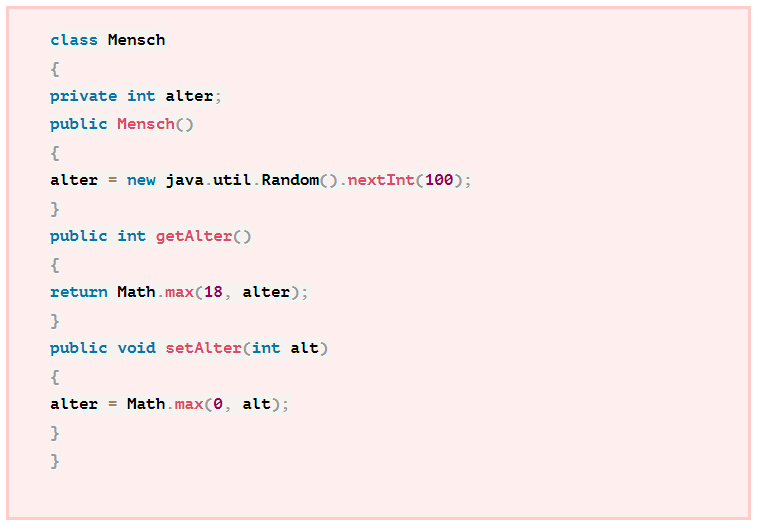
\includegraphics[width=11cm]{2.3.2.4/2.Entwicklung_des_Spiels/1-1.png}
\end{turn}
\end{figure}

\begin{itemize}
    \barrow je länger man überlebt, desto mehr Punkte erhält man
    \begin{itemize}
        \item Ziel: möglichst viele Punkte sammeln
    \end{itemize}
    \barrow mit der Leertaste kann ein Pfeil geschossen werden
    \begin{itemize}
        \item ein Schuss kostet einen Teil der Punktzahl
        \item wenn der Gegner getroffen wird, stirbt / verschwindet er
    \end{itemize}
    \newpage
    \barrow der Gegner schießt Stacheln
    \begin{itemize}
        \item wird der Spieler von einem Stachel getroffen, ist das Spiel vorbei
    \end{itemize}
    \barrow [die Geschwindigkeit von Greenfoot wird immer schneller, sodass sowohl alle Bewegungen als auch die Geschosse schneller werden]
    \barrow [wenn der Spieler stirbt, wird die erreichte Punktzahl ausgegeben]
\end{itemize}

\subsection{Klassenmodell}


\begin{figure}[ht]
	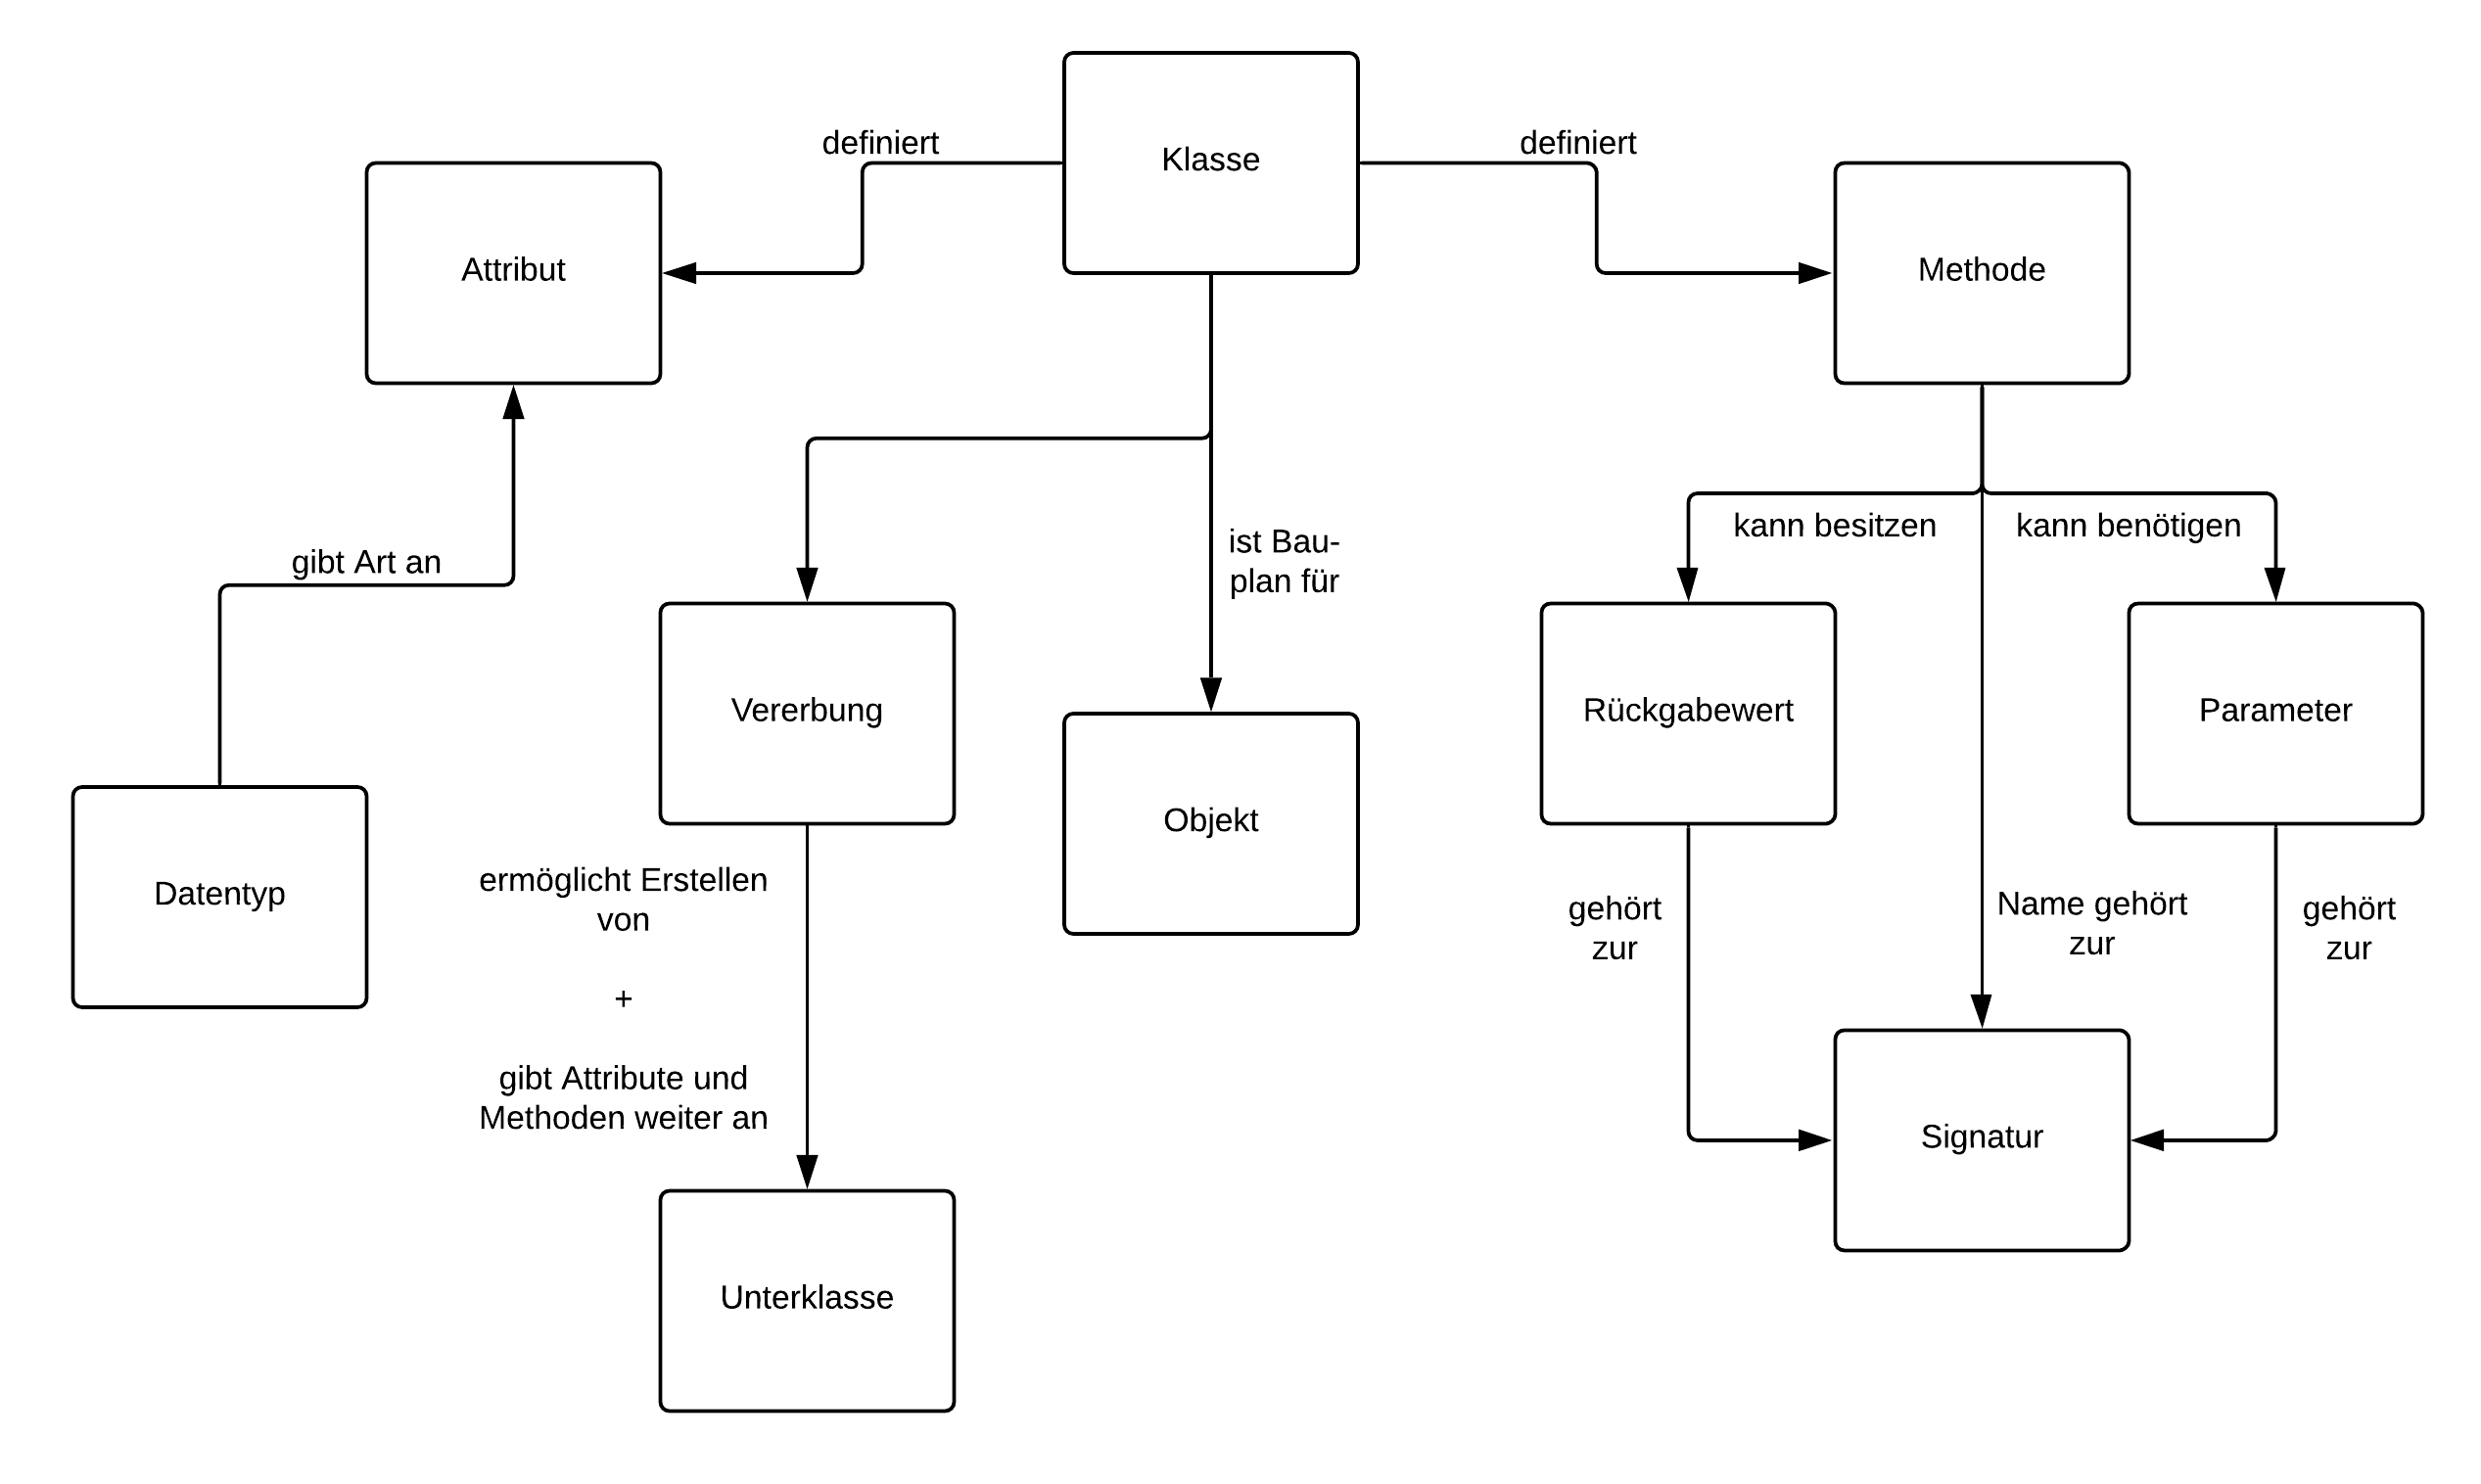
\includegraphics[width=8cm]{2.3.2.4/2.Entwicklung_des_Spiels/2-1.png}
	\hspace{0.5cm}
	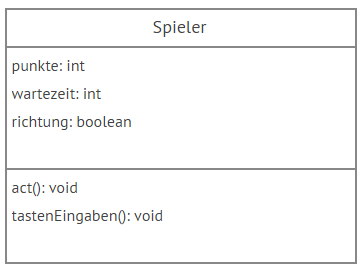
\includegraphics[width=8cm]{2.3.2.4/2.Entwicklung_des_Spiels/2-2.png}
\end{figure}

\begin{figure}[ht]
	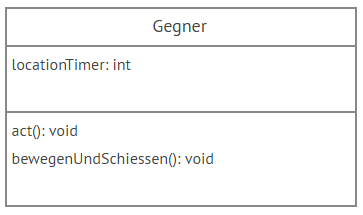
\includegraphics[width=8cm]{2.3.2.4/2.Entwicklung_des_Spiels/2-3.png}
	\hspace{0.5cm}
	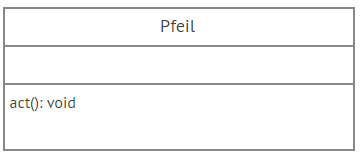
\includegraphics[width=8cm]{2.3.2.4/2.Entwicklung_des_Spiels/2-4.png}
\end{figure}

\begin{figure}[ht]
	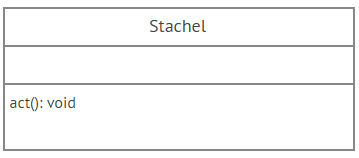
\includegraphics[width=8cm]{2.3.2.4/2.Entwicklung_des_Spiels/2-5.png}
\end{figure}

\newpage

\begin{itemize}
    \barrow \textbf{MyWorld}:
    \begin{itemize}
        \item \texttt{speed:} wird als Geschwindigkeit von Greenfoot gesetzt
        \item \texttt{speedTimer}: legt die Häufigkeit fest, wann die Geschwindigkeit sich erhöhen soll
        \item \texttt{spawnTimer}: legt die Häufigkeit vom Spawnen neuer Gegner fest
        \item \texttt{prepare}: fügt Spieler an festgelegter Stele hinzu
        \item \texttt{act}: hier wird die Geschwindigkeitsänderung und das Spawnen der Gegner aufgerufen
        \item \texttt{spawnGegner}: spawnt Gegner in einem von \texttt{spawnTimer} festgelegten Intervall
        \item \texttt{speedManager}: lässt die Geschwindigkeit immer schneller werden
    \end{itemize}
    \barrow \textbf{Spieler}:
    \begin{itemize}
        \item \texttt{punkte}: Punktestand des Spielers
        \item \texttt{wartezeit}: Intervall zwischen Schüssen
        \item \texttt{richtung}: passt sich der Bewegungsrichtung an
        \item \texttt{act}: aktualisiert Punktestand; wartet auf Tasten-Eingaben
        \item \texttt{tastenEingaben}: lässt bei Tastendruck etwas passieren (Bewegen, Schießen)
    \end{itemize}
    \barrow \textbf{Gegner}
    \begin{itemize}
        \item \texttt{locationTimer}: legt die Häufigkeit fest, wie oft sich Gegner bewegen und schießen
        \item \texttt{act}: ruft Bewegung und Schießvorgang auf
        \item \texttt{bewegenUndSchiessen}: Bewegung und Schießvorgang
    \end{itemize}
    \barrow \textbf{Pfeil / Stachel}
    \begin{itemize}
        \item \texttt{act}: überprüft Berührung mit Gegner / Spieler oder ob es am Ende der Welt ist
    \end{itemize}
\end{itemize}

\subsection{Programm}

Da dieses Projekt schon etwas komplexer ist, ist mein fertiger Projektordner \href{https://github.com/cyb3rko/inf-schule-loesungen/raw/master/2/2.3/2.3.2/2.3.2.4\%20Space\%20Invaders/2.Entwicklung_des_Spiels/Space\%20Invaders.zip}{HIER} herunterzuladen.\\
Beim Implementieren der gestellten Funktionen gehen wir am besten chronologisch durch.

Angefangen habe ich mit dem simplen Bewegen des Spielers, was auch schon Teil vorheriger Projekte war:\\
\begin{lstlisting}
void tastenEingaben() {
    if (Greenfoot.isKeyDown("left")) {
        if (richtung) {
            getImage().mirrorHorizontally();
        }

        richtung = false;
        setLocation(getX() - 10, getY());
    }

    if (Greenfoot.isKeyDown("right")) {
        if (!richtung) {
            getImage().mirrorHorizontally();
        }

        richtung = true;
        setLocation(getX() + 10, getY());
    }
}
\end{lstlisting}

Damit es nicht so seltsam aussieht, wird der Spieler je nach Laufrichtung an der Y-Achse gespiegelt. Der Rest müsste klar sein...

Der nächste Punkt wäre die Punkteverwaltung:\\
Bei jedem Aufruf der \texttt{act}-Methode wird die Punktzahl also einfach um eins erhöht, außerdem wollen wir es direkt anzeigen lassen.\\
Eingefügt in den Code sieht das in der Spieler-Klasse dann so aus:

\newpage

\begin{lstlisting}
public void act() {
    getWorld().showText("Punktestand: " + punkte, 110, 30);
    punkte++;
}
\end{lstlisting}

Mit den Koordinaten der Textausgabe muss man einfach ein wenig herumprobieren, bis man etwas Sinnvolles gefunden hat.

Damit wäre schon die zweite Funktion fertig, die nächste folgt zugleich. Diese fordert, dass ein Pfeil bei Drücken der Leertaste nach oben geschossen wird.\\
Der Schuss soll Punkte kosten und bei Kontakt mit einem Gegner soll dieser sterben / verschwinden.\\
Wir fügen zu der Abfrage der Tasteneingaben noch die Leertaste hinzu und erstellen bei Klick dieser einen neuen Pfeil über dem Spieler, außerdem ziehen wir ein paar Punkte ab:\\
\begin{lstlisting}
void tastenEingaben() {
        ...

        if (Greenfoot.isKeyDown("space") && wartezeit > 20) {
            getWorld().addObject(new Pfeil(), getX(), 555);

            punkte -= 30;
            wartezeit = 0;
        }
    }
\end{lstlisting}

Damit der Pfeil sich nun auch bewegt und bei Kontakt etwas ausführt, wechseln wir zu der \texttt{Pfeil}-Klasse. Dort wird in der \texttt{act}-Methode bei Kontakt mit einem Gegner der Gegner und der Pfeil entfernt. Solange der Rand der Welt nicht erreicht ist, bewegt sich der Pfeil stetig nach oben. Bei Berühung des Randes der Welt wird der Pfeil auch entfernt:

\newpage

\begin{lstlisting}
public void act() {
        if (isTouching(Gegner.class)) {
            removeTouching(Gegner.class);
            getWorld().removeObject(this);
        } else if (!isAtEdge()) {
            setLocation(getX(), getY() - 10);
        } else {
            getWorld().removeObject(this);
        }
    }  
\end{lstlisting}


Ziemlich ähnlich läuft das auch mit den Stacheln der Gegner ab.\\
Zuerst wird ein Stachel in gewissen Abständen von einem Gegner gespawnt:\\

\begin{lstlisting}
void bewegenUndSchiessen() {
    setLocation(random.nextInt(1280), getY());
    getWorld().addObject(new Stachel(), getX(), 150);
}
\end{lstlisting}

Die Bewegung des Stachels steht in der \texttt{Stachel}-Klasse:\\

\begin{lstlisting}
public void act() {
    if (!isAtEdge()) {
        setLocation(getX(), getY() + 10);
    } else {
        getWorld().removeObject(this);
    }
}
\end{lstlisting}

Dieser Code müsste auch verständlich sein...

Nun wollen wir noch das Spiel beenden lassen, falls ein Stachel den Spieler trifft, dazu packen wir folgenden Code einfach noch mit in die \texttt{act}-Methode des Spielers:\\

\begin{lstlisting}
if (isTouching(Stachel.class)) {
    Greenfoot.stop();
}
...
\end{lstlisting}


Nun haben wir die Hauptfunktionen des Spiels fertig.\\
Widmen wir uns noch den beiden optionale Funktionen. Die erste ist das Größerwerden der Geschwindigkeit.\\
Dieses Problem gehen wir in der \texttt{MyWorld}-Klasse an, da diese sozusagen die oberste Instanz ist, weil sie die anderen Objekte wie z.B. Spieler, Gegner etc. zur Welt hinzufügt.\\
Wir ergänzen dort dann folgende Methode:\\

\begin{lstlisting}
void speedManager() {
    speedTimer--;
    
    if (speedTimer == 0) {
        speed++;
        Greenfoot.setSpeed(speed);
        speedTimer = 200;
    }
    }
\end{lstlisting}

Wenn diese Methode nun immer wieder (indirekt über die \texttt{act}-Methode) von Greenfoot aufgerufen wird, passt sich die Geschwindigkeit von alleine an.

Der letzte Punkt ist die Ausgabe der Punktzahl, wenn das Spiel beendet wird.\\
Dazu fügen wir einen Schnipsel aus dem Bereich \href{https://www.inf-schule.de/programmierung/oopjava/anhang}{"Tipps und Tools"} direkt auf \texttt{inf-schule.} in die \texttt{act}-Methode ein:

\newpage

\begin{lstlisting}
if (isTouching(Stachel.class)) {
    JOptionPane.showMessageDialog(null, "Du hast " + punkte + " Punkte erreicht.");
    Greenfoot.stop();
}
...
\end{lstlisting}

\subsection{Spielen}

Zu dieser Aufgabe sind meines Erachtens nach keine Anleitungen und/oder Erläuterungen nötig.\\
Wenn doch Fragen aufkommen, schreib' einfach an \textbf{\href{mailto:niko@cyb3rko.de}{niko@cyb3rko.de}}.

\section{Fachkonzept-Softwareentwicklungsphasen}

Zu dieser Seite sind meines Erachtens nach keine Anleitungen und/oder Erläuterungen nötig.\\
Wenn doch Fragen aufkommen, schreib' einfach an \textbf{\href{mailto:niko@cyb3rko.de}{niko@cyb3rko.de}}.

\end{document}
